\documentclass{article}
\usepackage[utf8]{inputenc}
\pagenumbering{Roman}
\usepackage{ragged2e}
\usepackage{graphicx}
\usepackage{wrapfig}
\usepackage[spanish]{babel}
\usepackage{hyperref}
\usepackage{datetime}


\begin{document}


\title{\huge \textbf{Instructivo para la extracción de datos de monitor de signos vitales y BIS } \vspace{8cm}}
\author{Carlos Valle \\ \href{mailto:cgvalle@uc.cl}{cgvalle@uc.cl} }
\date{21 de Febrero 2024}
\maketitle


\newpage

\section{Motivación}

El objetivo de este instructivo es guiar en el setup de equipos y software para la extración de datos del monitor de signos vitales \href{https://www.gehealthcare.com/products/patient-monitoring/patient-monitors/carescape-monitor-b650}{Carescape B650} y el monitor \href{https://www.medtronic.com/covidien/es-cl/products/brain-monitoring/bis-complete-4-channel-monitor.html}{Bis vista}.

Los procedimientos para obtener los datos de ambos equipos son independientes por lo que se abordaran en dos secciones independientes, pero se recomienda realizarlo uno a la vez. En cada sección se describirá el setup, así como el uso del software necesario. 

Los códigos y archivos necesarios se encuentran alojados en la carpeta de GitHub: \url{https://github.com/cgvalle/monitor_signos_vitales} 



\newpage



% B650
\section{Monitor Carescape B650}
Para la extracción de las señales fisiológicas durante cirugia se utiliza el monitor Carescape B650 (Fig. \ref{fig:b650_frontal}). Los códigos e instructivos se basan en dicho monitor, por lo que no se asegura la compatibilidad con un tercero. 

\begin{figure}[h]
	\centering
    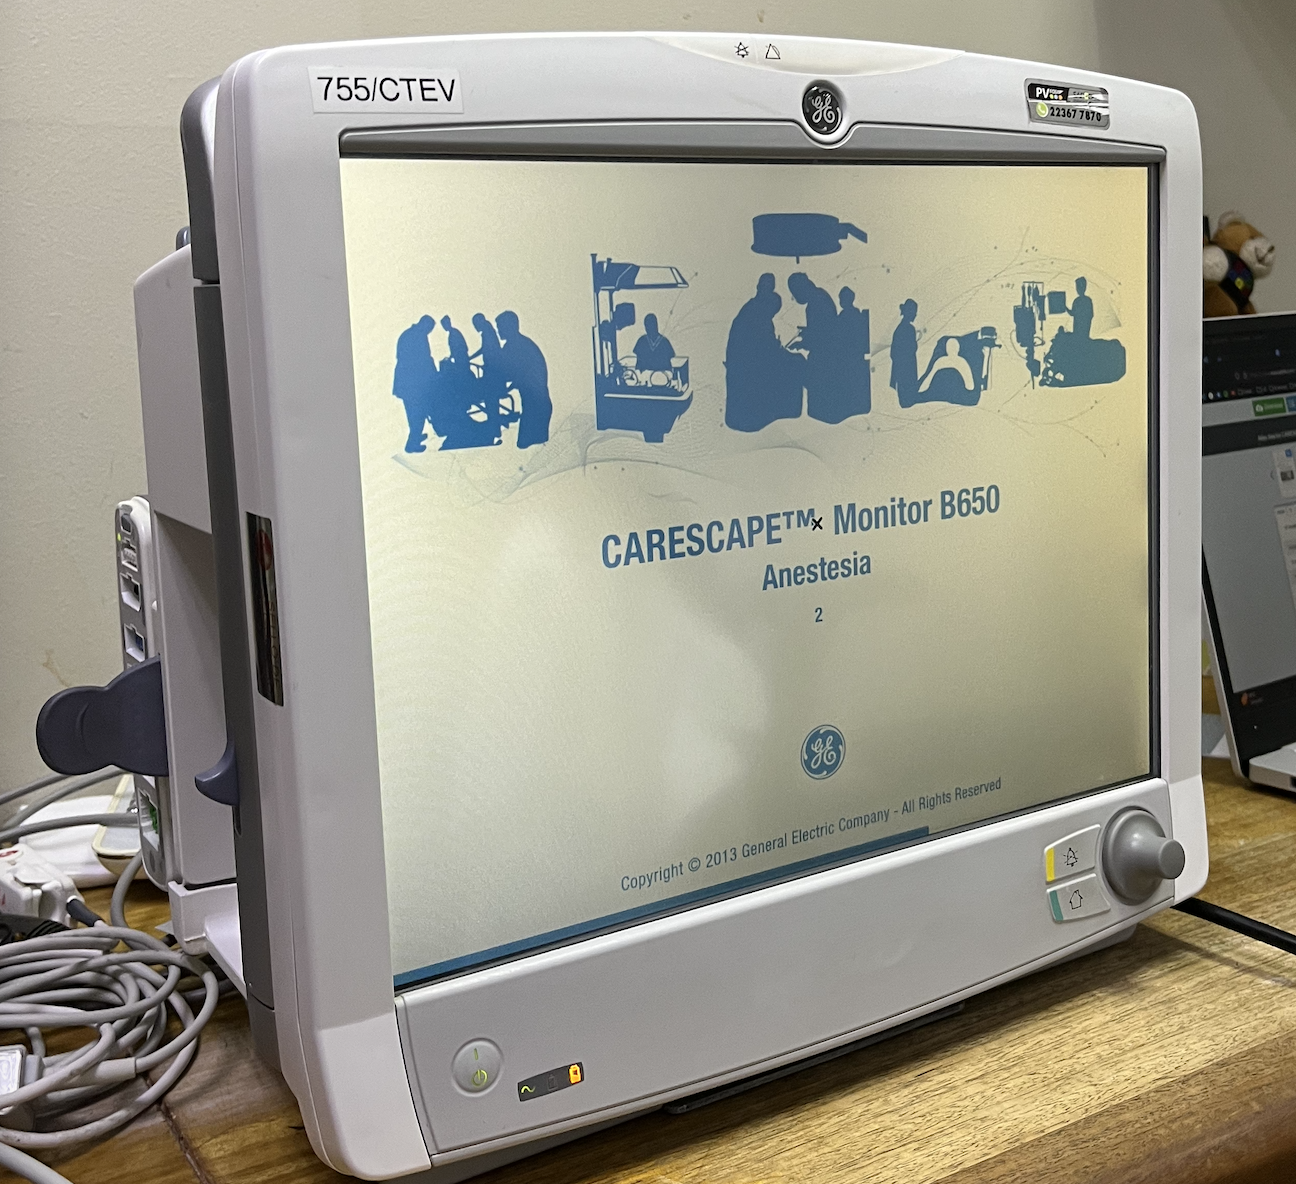
\includegraphics[scale=0.6]{img/carescape_b650.jpeg}
    \caption{Vista frontal monitor Carescape B650}
    \label{fig:b650_frontal}
\end{figure}

\subsection{Preparativos}
Antes de comenzar es necesario configurar el monitor para que envíe los datos a un computador, cambiando la configuración de red (Network Type) a S/5 Collect. Para esto se debe seguir el siguiente procedimiento:

\begin{enumerate}
	\item Encender el monitor y esperar a que cargue.
	\item Ir a la pantalla de Config. Monitor y seleccionar configuración. 
	\item Se le solicitara un usuario y contraseña. Los valores por defecto son: para usuario \textbf{biomed} y la contraseña es \textbf{Change Me}. Si no funcionan, contactar al servicio TI del hospital para obtener las credenciales.
	\item Una vez dentro de la configuración, seleccionar la pestaña de red y cambiar el Network Type a S/5 (Fig. \ref{fig:network_type}). Luego dar click en next
	
	\begin{figure}[h]
		\centering
		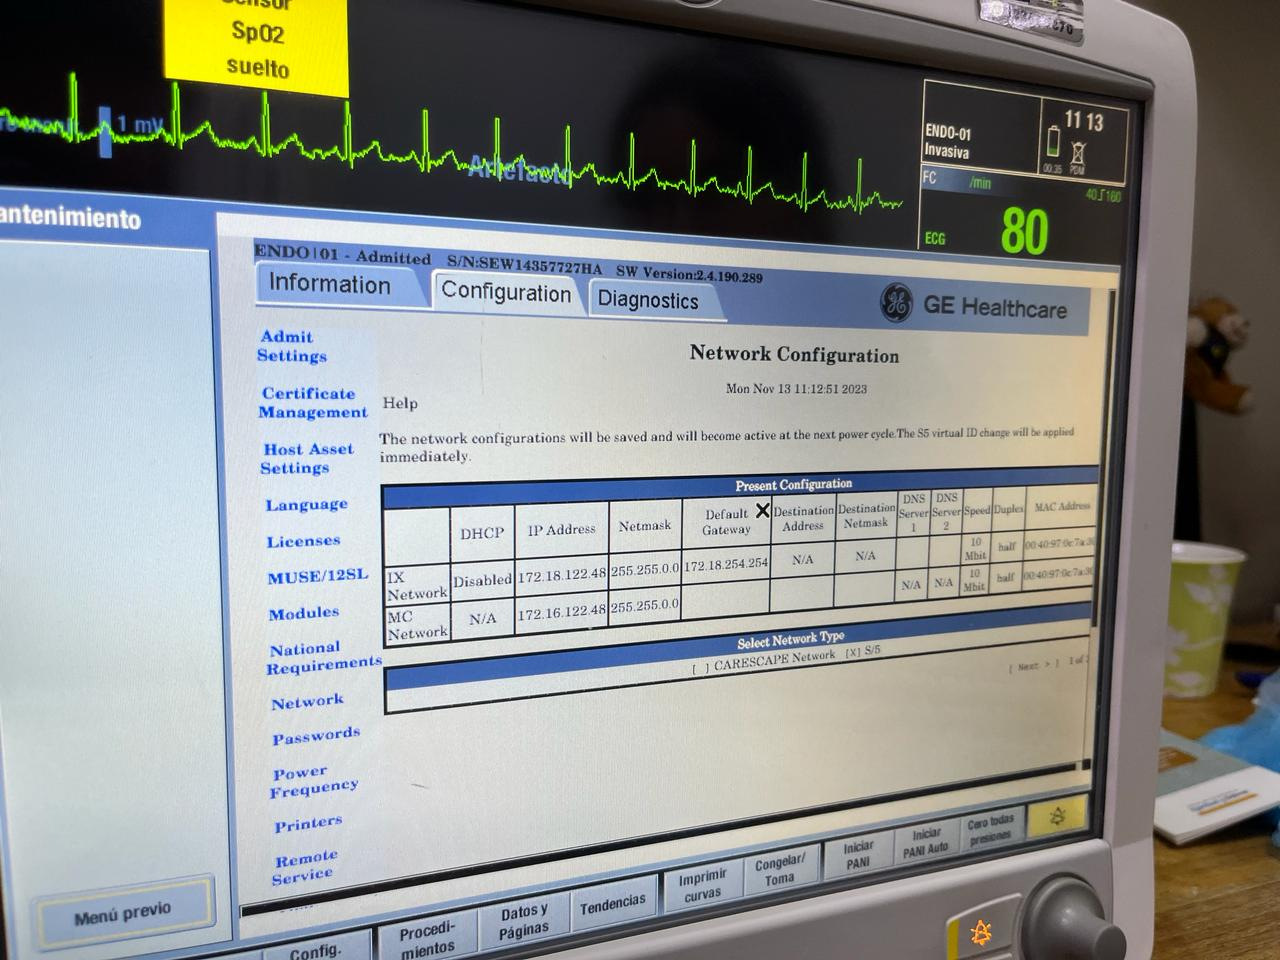
\includegraphics[scale=0.3]{img/network.png}
		\caption{Red configurada en S/5}
		\label{fig:network_type}
	\end{figure}

	\item En el apartado de Virtual ID utilizar el numero 50001 o mayor (Fig. \ref{fig:virtual_id}). 
	
	\begin{figure}[h]
		\centering
		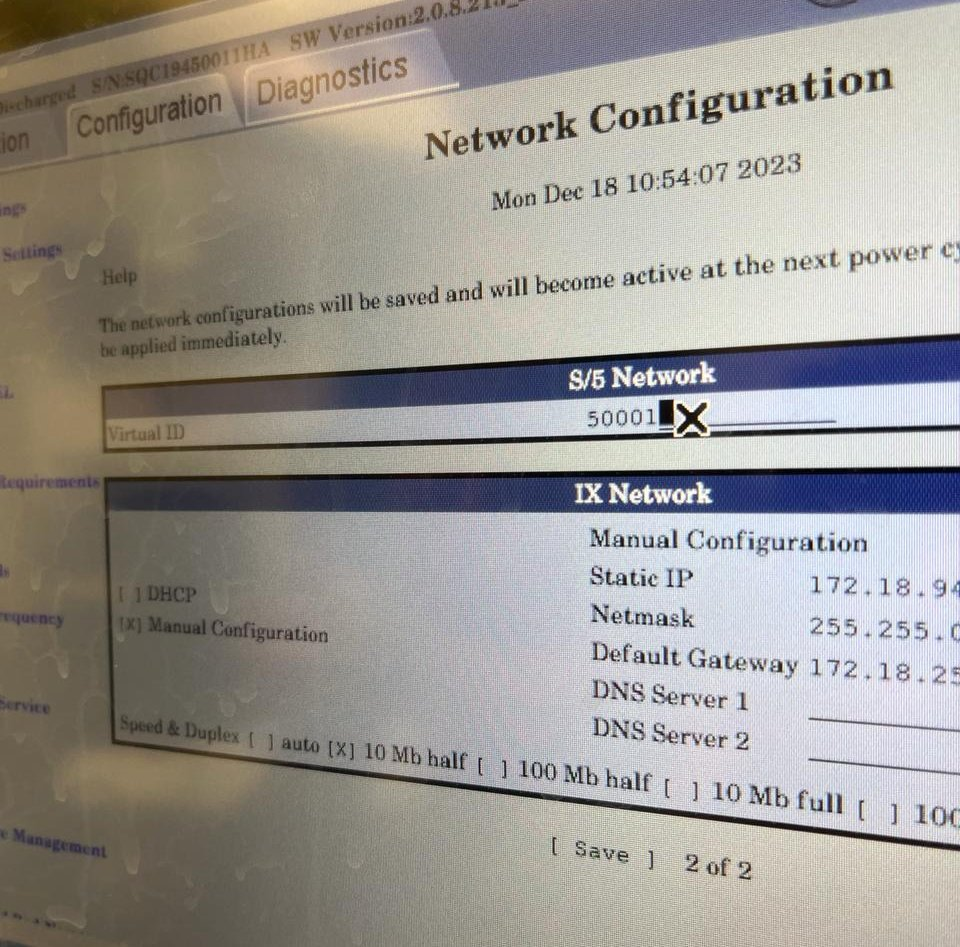
\includegraphics[scale=0.3]{img/network_id.jpeg}
		\caption{Virtual ID}
		\label{fig:virtual_id}
	\end{figure}
	\item Guardar los cambios y reiniciar el monitor.
	\item Cambiar fecha y hora del monitor, para que coincida con la del computador al que se conectará incluidos los segundos.

\end{enumerate}

Es importante hacer notas que este proceso puede variar dependiendo de la versión del software del monitor, pero en general el proceso es similar aunque con variaciones en la interfas. 






\subsection{Setup}
Cables necesarios:

\begin{enumerate}
	\item Cable ATEN USB to Serial RS232.  (Es necesario que cuente con el chip VID 0557, modelos mas nuevos vienen con 067b. De necesitar otro, buscarlo en ebay priorizando el más viejo que exista para aumentar las probabilidades de que venga con el chip VID 0557)

	\includegraphics*[scale=0.12]{img/ATEN_USB.jpeg}
	\item  Cable RS232 hembra hembra 

	\includegraphics*[scale=0.12]{img/rs232_hembra_hembra.jpeg}
	\item Cable RS232 a usb (Null Modem)

	\includegraphics*[scale=0.12]{img/rs232_macho_a_usb.jpeg}

\end{enumerate}

Se conectan los 3 cables en serie, quedando con dos extremos USB. El USB del cable 3 se conecta al computador y el USB del cable 1 se conecta al monitor. Es necesario que este utilmo se conecte al monitor mediante la entrada USB inferior derecha, tal como se ve en la imagen.

\begin{figure}[h]
	\centering
	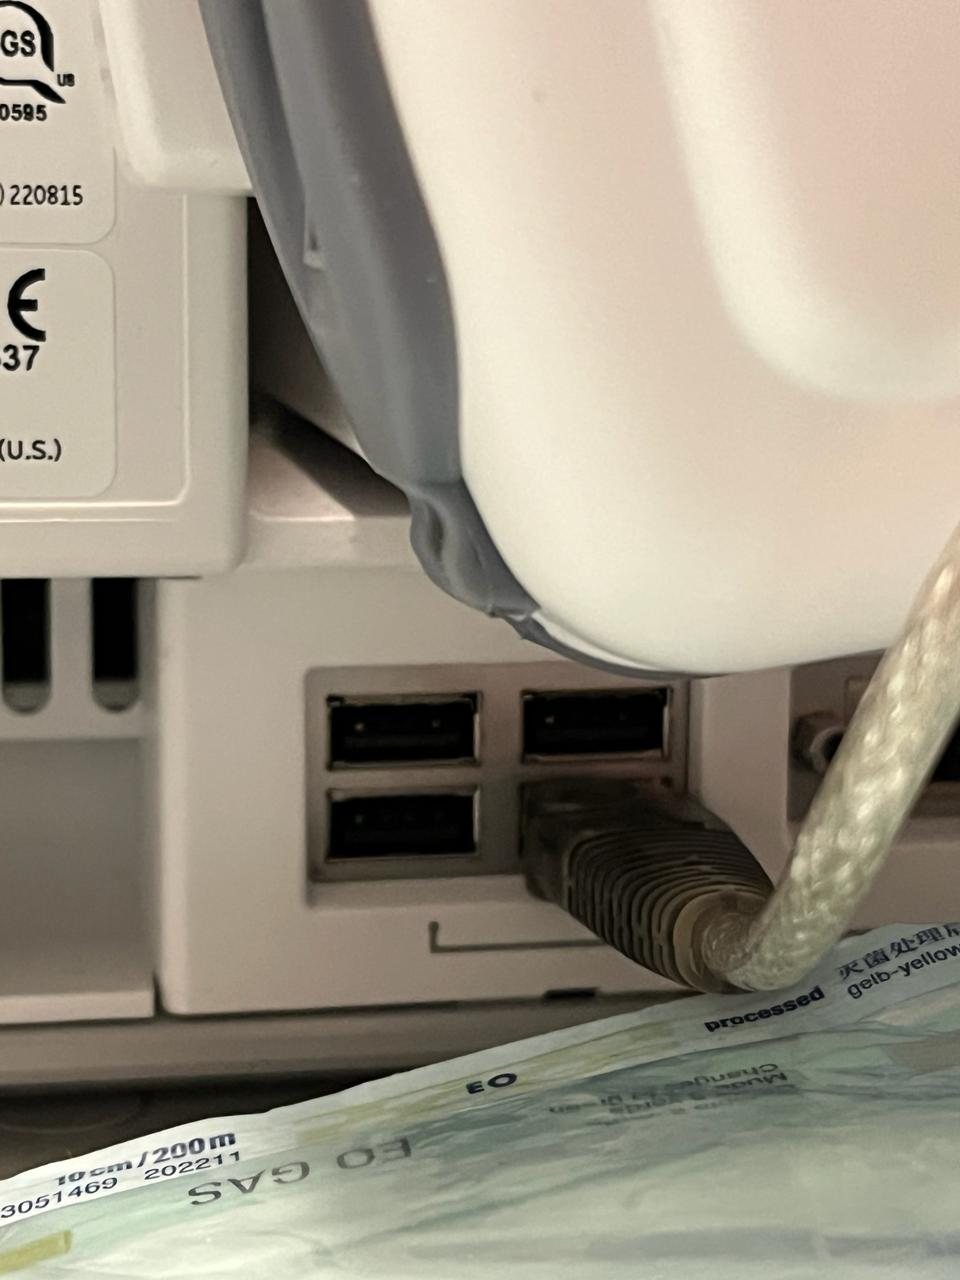
\includegraphics[scale=0.2]{img/b650_rear_panel.png}
	\caption{Vista posterior monitor Carescape B650. Solo se debe usar el usb inferior derecho.}
	\label{fig:b650_posterior}
\end{figure}

El otro extremo, puede ir conectado a cualquier puerto USB del computador.



\subsection{Uso}
Clonar el repositorio de Github: \url{https://github.com/cgvalle/monitor_signos_vitales}. En la carpeta \textbf{monitor\_record} encontraras dos archivos:
\begin{itemize}
	\item \textbf{VSCapture.exe}: Este programa se encarga de capturar los datos del monitor y guardarlos en un archivo .csv.
	\item \textbf{README.md}: Instructivo rapido de uso.
\end{itemize}

Una vez iniciado VSCapture, debera escribir el puerto COM al que esta conectado el monitor. Si solo esta conectado un dispositivo, el puerto COM sera el que se muestra en la lista. Si no, debera buscarlo en el administrador de dispositivos de Windows. Debera selecionar el intervalo de transmision de datos, el cual se recomienda que sea de 1 segundo. Finalmente, se le pedira que indique el tipo de data que quiere capturar entre 5 opciones. Este proceso se encuentra representado en la Fig. \ref{fig:vs_capture}.


\begin{figure}[h]
	\centering
	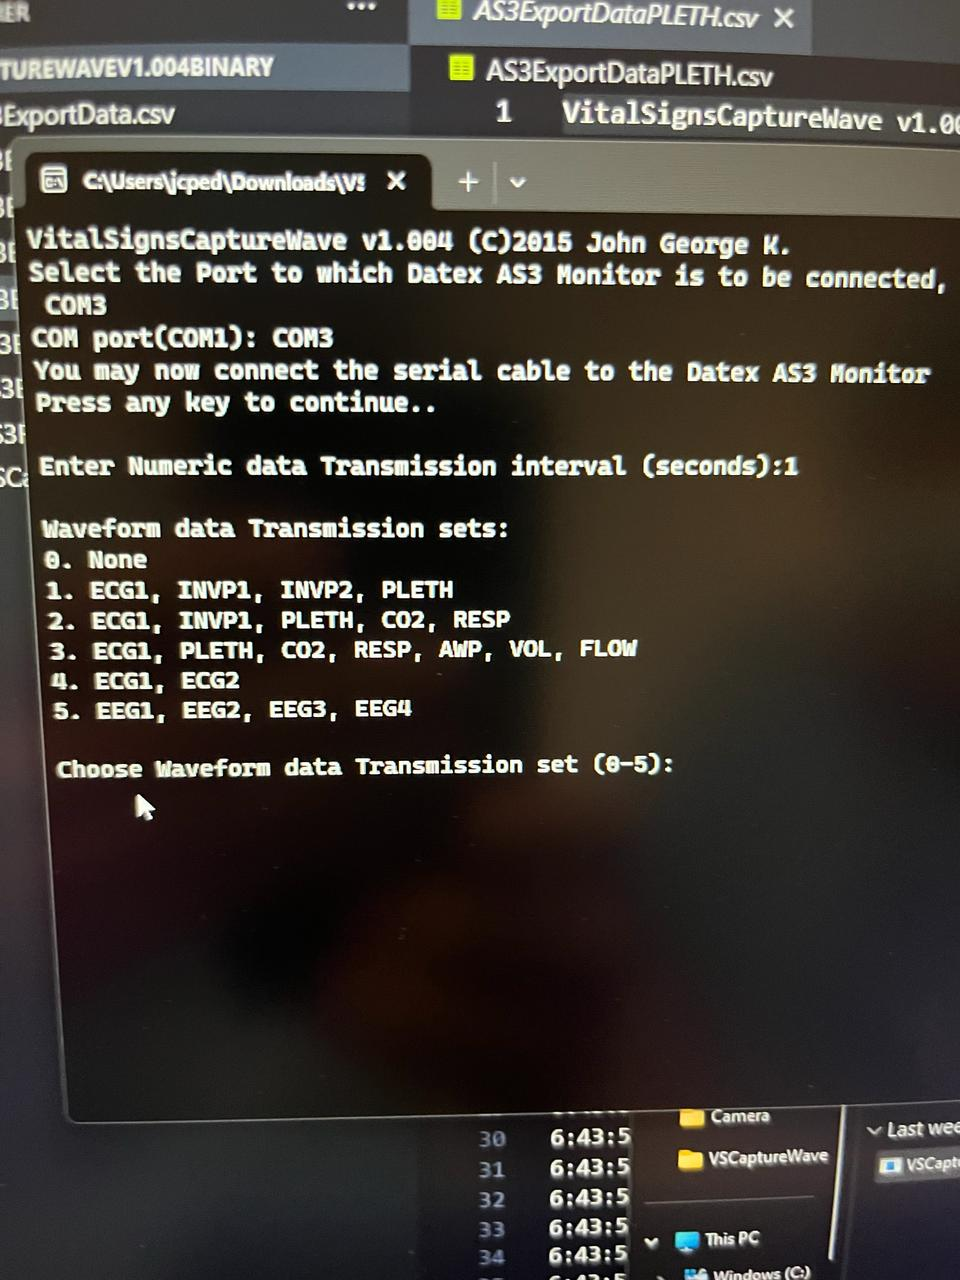
\includegraphics[scale=0.2]{img/vs_capture.png}
	\caption{Proceso de captura de datos con VSCapture.}
	\label{fig:vs_capture}
\end{figure}


Al finalizar la cirugia, se debe presionar el botón de ESCAPE en la terminal del programa para que se terminar con la adquisición. Este archivo se guardara en la carpeta \textbf{monitor\_record} con el nombre de \textbf{*.csv}.



\section{Monitor BIS Vista}

El monitor BIS Vista (Fig. \ref{fig:bis_frontal}) es un monitor de electroencefalografía que se utiliza para medir el nivel de conciencia del paciente. 

\begin{figure}[h]
	\centering
	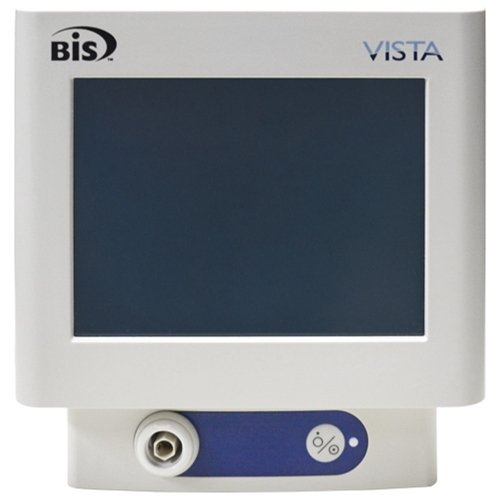
\includegraphics[scale=0.2]{img/bis_vista.png}
	\caption{Vista frontal monitor BIS Vista}
	\label{fig:bis_frontal}
\end{figure}



\subsection{Preparativos}
De manera similar al monitor Carescape B650, es necesario configurar la hora (incluyendo segundos) y fecha del monitor para que coincida con la del computador al que se conectará. Es importante que este paso se realice de manera correcta, ya que de lo contrario los datos estaran desfasados.

\subsection{Setup}

Elementos necesarios:

\begin{enumerate}
	\item Cable RS232 macho a usb (se recomienda el modelo Trendnet TU-S9)
	\item Cable RS232 macho hembra
	\item Pendrive USB 
\end{enumerate}

Se conectan ambos cables en serie, quedando con un extremo USB. El USB del cable se conecta al computador y el otro extremo se conecta al monitor. El pendrive se conecta al puerto USB del monitor (Fig. \ref{fig:bis_rear_panel}).


\begin{figure}
	\centering
    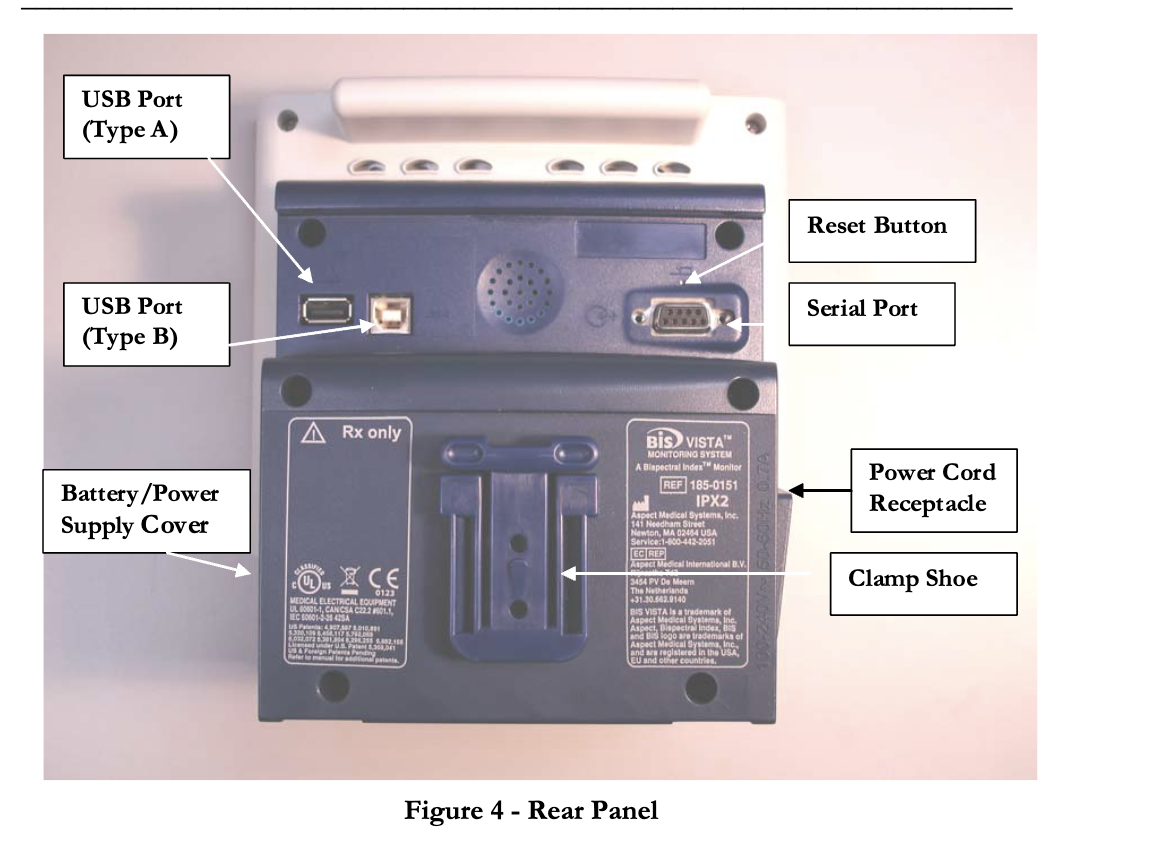
\includegraphics[scale=0.5]{img/bis_rear_panel.png}
    \caption{Caption}
	\label{fig:bis_rear_panel}
\end{figure}


\subsection{Uso}

Luego de conectar el cintillo al paciente y que la señal se estabilice, se debe presionar el botón de exportar datos de manera continua en el monitor. De esta forma se guardaran los datos en el pendrive. 

Clonar el repositorio de Github: \url{https://github.com/cgvalle/monitor_signos_vitales}. En la carpeta \textbf{bis\_record} encontraras dos archivos:

\begin{itemize}
	\item \textbf{main.py}: Este programa se encargara de enviar marcadores al monitor para que se guarden en el pendrive.
	\item \textbf{config.json }: Archivo de configuración que contiene con que tecla se envia el marcador.
	\item \textbf{output.txt} : Archivo donde se guardaran los marcadores enviados.
	\item \textbf{README.md}: Instructivo rapido de uso.
\end{itemize}


Para ejecutar el programa, se debe abrir una terminal en la carpeta \textbf{bis\_record} y ejecutar el comando \textbf{python main.py}. El programa le pedira que presione la tecla que se encuentra en el archivo de configuración. Cada vez que presione la tecla, se guardara un marcador en el archivo \textbf{output.txt} y en el pendrive. Se le dara a elegir el puerto COM al que esta conectado el monitor. Si solo esta conectado un dispositivo, el puerto COM sera el que se muestra en la lista. Si no, debera buscarlo en el administrador de dispositivos de Windows.

Para finalizar la adquisición, se debe cerrar la ventana del programa. 





\end{document}
